\subsection{Grafos e Convexidades}
\begin{frame}{Convexidade em Grafos}
A \textit{convexidade} em um grafo $G$ é dada por um conjunto ${\cal C}$, formado por subconjuntos de $V(G)$ que:
\begin{itemize}
    \item$\emptyset,V(G) \in {\cal C}$
    \item ${\cal C}$ é um conjunto fechado em relação a operação de intersecção
    \item Cada elemento de ${\cal C}$ é um \textit{conjunto convexo}
\end{itemize}
Tipo especial de convexidade são as convexidades definidas por um conjunto ${\cal P}$ de caminhos em grafos. 
\textit{Convexidade geodésica} é quando ${\cal P}$ é o conjunto de todos os menores caminhos.
\textit{Convexidade $P_3$} é quando ${\cal P}$ é o conjunto de todos os caminhos com três vértices.
\end{frame}

% ----------------- NOVO SLIDE --------------------------------
\subsection{Convexidade $P_3$}
\begin{frame}
\frametitle{Convexidade $P_3$}
%\framesubtitle{Envoltória Convexa}
  \begin{columns}[T]
    \begin{column}{.5\textwidth}
    \centering
    \resizebox{\textwidth}{!}{%
        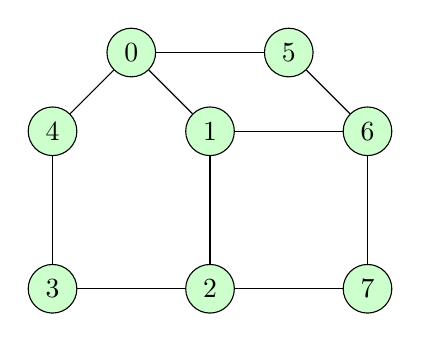
\begin{tikzpicture}[auto,node_style/.style={circle,draw=black,fill=green!20!},
           node_style_selected/.style={circle,draw=black,fill=red!20!},edge_style/.style={draw=black}]
            \node[node_style] (v0) at (1, 3)  {0};
            \node[node_style] (v1) at (2, 2)  {1};
            \node[node_style] (v2) at (2, 0)  {2};
            \node[node_style] (v3) at (0, 0)  {3};
            \node[node_style] (v4) at (0, 2)  {4};
            \node[node_style] (v5) at (3, 3)  {5};
            \node[node_style] (v6) at (4, 2)  {6};
            \node[node_style] (v7) at (4, 0)  {7};
            \draw[edge_style]  (v0) edge node{} (v1);
            \draw[edge_style]  (v1) edge node{} (v2);
            \draw[edge_style]  (v2) edge node{} (v3);
            \draw[edge_style]  (v2) edge node{} (v7);
            \draw[edge_style]  (v3) edge node{} (v4);
            \draw[edge_style]  (v4) edge node{} (v0);
            \draw[edge_style]  (v0) edge node{} (v5);
            \draw[edge_style]  (v1) edge node{} (v6);
            \draw[edge_style]  (v5) edge node{} (v6);
            \draw[edge_style]  (v6) edge node{} (v7);
        \end{tikzpicture}
    }
    \end{column}
    \begin{column}{.5\textwidth}
     \begin{itemize}
        \item{$V(G) = \{0, 1, 2, 3, 4, 5, 6, 7\}$}
        \item{$E(G) = \{(0,1), (1,2), (1,6), (2,3),$ $(3,4),(4,0), (0,5), (5,6), (6,7)\}$}
     \end{itemize}
    \end{column}
  \end{columns}
\end{frame}

\begin{frame}
\frametitle{Convexidade $P_3$}
%\framesubtitle{Envoltória Convexa}
  \begin{columns}[T]
    \begin{column}{.5\textwidth}
    \centering
    \resizebox{\textwidth}{!}{%
        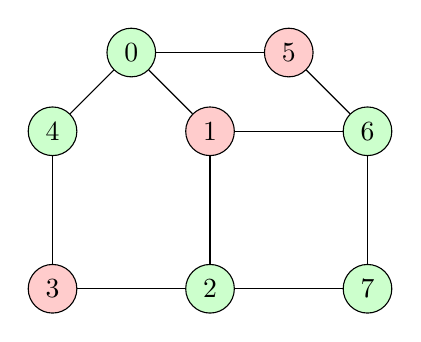
\begin{tikzpicture}[auto,node_style/.style={circle,draw=black,fill=green!20!},
           node_style_selected/.style={circle,draw=black,fill=red!20!},
           node_style_selected2/.style={circle,draw=black,fill=yellow!20!},
           edge_style/.style={draw=black}]
            \node[node_style] (v0) at (1, 3)  {0};
            \node[node_style_selected] (v1) at (2, 2)  {1};
            \node[node_style] (v2) at (2, 0)  {2};
            \node[node_style_selected] (v3) at (0, 0)  {3};
            \node[node_style] (v4) at (0, 2)  {4};
            \node[node_style_selected] (v5) at (3, 3)  {5};
            \node[node_style] (v6) at (4, 2)  {6};
            \node[node_style] (v7) at (4, 0)  {7};
            \draw[edge_style]  (v0) edge node{} (v1);
            \draw[edge_style]  (v1) edge node{} (v2);
            \draw[edge_style]  (v2) edge node{} (v3);
            \draw[edge_style]  (v2) edge node{} (v7);
            \draw[edge_style]  (v3) edge node{} (v4);
            \draw[edge_style]  (v4) edge node{} (v0);
            \draw[edge_style]  (v0) edge node{} (v5);
            \draw[edge_style]  (v1) edge node{} (v6);
            \draw[edge_style]  (v5) edge node{} (v6);
            \draw[edge_style]  (v6) edge node{} (v7);
        \end{tikzpicture}
    }
    \end{column}
    \begin{column}{.5\textwidth}
     $S = \{1, 3, 5\}$ É Convexo?

     Não
    \end{column}
  \end{columns}
\end{frame}

\begin{frame}
\frametitle{Convexidade $P_3$}
\framesubtitle{Envoltória Convexa}
  \begin{columns}[T]
    \begin{column}{.5\textwidth}
    \centering
    \resizebox{\textwidth}{!}{%
        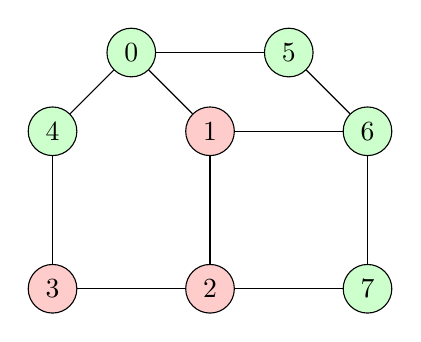
\begin{tikzpicture}[auto,node_style/.style={circle,draw=black,fill=green!20!},
           node_style_selected2/.style={circle,draw=black,fill=yellow!20!},
           node_style_selected/.style={circle,draw=black,fill=red!20!},
           edge_style/.style={draw=black}]
            \node[node_style] (v0) at (1, 3)  {0};
            \node[node_style_selected] (v1) at (2, 2)  {1};
            \node[node_style_selected] (v2) at (2, 0)  {2};
            \node[node_style_selected] (v3) at (0, 0)  {3};
            \node[node_style] (v4) at (0, 2)  {4};
            \node[node_style] (v5) at (3, 3)  {5};
            \node[node_style] (v6) at (4, 2)  {6};
            \node[node_style] (v7) at (4, 0)  {7};
            \draw[edge_style]  (v0) edge node{} (v1);
            \draw[edge_style]  (v1) edge node{} (v2);
            \draw[edge_style]  (v2) edge node{} (v3);
            \draw[edge_style]  (v2) edge node{} (v7);
            \draw[edge_style]  (v3) edge node{} (v4);
            \draw[edge_style]  (v4) edge node{} (v0);
            \draw[edge_style]  (v0) edge node{} (v5);
            \draw[edge_style]  (v1) edge node{} (v6);
            \draw[edge_style]  (v5) edge node{} (v6);
            \draw[edge_style]  (v6) edge node{} (v7);
        \end{tikzpicture}
    }
    \end{column}
    \begin{column}{.5\textwidth}
     $S = \{1, 2, 3\}$ É Convexo?

     Sim
    \end{column}
  \end{columns}
\end{frame}

\begin{frame}
\frametitle{Convexidade $P_3$}
\framesubtitle{Envoltória Convexa}
  \begin{columns}[T]
    \begin{column}{.5\textwidth}
    \centering
    \resizebox{\textwidth}{!}{%
        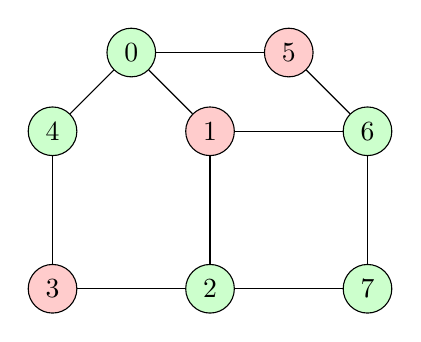
\begin{tikzpicture}[auto,node_style/.style={circle,draw=black,fill=green!20!},
           node_style_selected/.style={circle,draw=black,fill=red!20!},
           node_style_selected2/.style={circle,draw=black,fill=yellow!20!},
           edge_style/.style={draw=black}]
            \node[node_style] (v0) at (1, 3)  {0};
            \node[node_style_selected] (v1) at (2, 2)  {1};
            \node[node_style] (v2) at (2, 0)  {2};
            \node[node_style_selected] (v3) at (0, 0)  {3};
            \node[node_style] (v4) at (0, 2)  {4};
            \node[node_style_selected] (v5) at (3, 3)  {5};
            \node[node_style] (v6) at (4, 2)  {6};
            \node[node_style] (v7) at (4, 0)  {7};
            \draw[edge_style]  (v0) edge node{} (v1);
            \draw[edge_style]  (v1) edge node{} (v2);
            \draw[edge_style]  (v2) edge node{} (v3);
            \draw[edge_style]  (v2) edge node{} (v7);
            \draw[edge_style]  (v3) edge node{} (v4);
            \draw[edge_style]  (v4) edge node{} (v0);
            \draw[edge_style]  (v0) edge node{} (v5);
            \draw[edge_style]  (v1) edge node{} (v6);
            \draw[edge_style]  (v5) edge node{} (v6);
            \draw[edge_style]  (v6) edge node{} (v7);
        \end{tikzpicture}
    }
    \end{column}
    \begin{column}{.5\textwidth}
     $S = \{1, 3, 5\}$ É Convexo?
    \end{column}
  \end{columns}
\end{frame}

\begin{frame}
\frametitle{Convexidade $P_3$}
\framesubtitle{Envoltória Convexa}
  \begin{columns}[T]
    \begin{column}{.5\textwidth}
    \centering
    \resizebox{\textwidth}{!}{%
        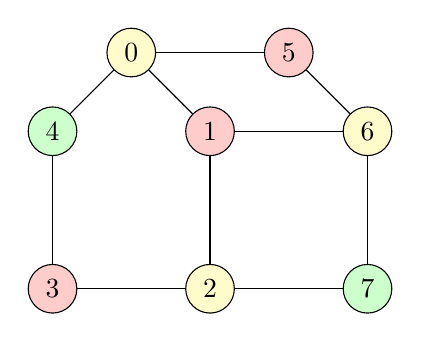
\begin{tikzpicture}[auto,node_style/.style={circle,draw=black,fill=green!20!},
           node_style_selected/.style={circle,draw=black,fill=red!20!},
           node_style_selected2/.style={circle,draw=black,fill=yellow!20!},
           edge_style/.style={draw=black}]
            \node[node_style_selected2] (v0) at (1, 3)  {0};
            \node[node_style_selected] (v1) at (2, 2)  {1};
            \node[node_style_selected2] (v2) at (2, 0)  {2};
            \node[node_style_selected] (v3) at (0, 0)  {3};
            \node[node_style] (v4) at (0, 2)  {4};
            \node[node_style_selected] (v5) at (3, 3)  {5};
            \node[node_style_selected2] (v6) at (4, 2)  {6};
            \node[node_style] (v7) at (4, 0)  {7};
            \draw[edge_style]  (v0) edge node{} (v1);
            \draw[edge_style]  (v1) edge node{} (v2);
            \draw[edge_style]  (v2) edge node{} (v3);
            \draw[edge_style]  (v2) edge node{} (v7);
            \draw[edge_style]  (v3) edge node{} (v4);
            \draw[edge_style]  (v4) edge node{} (v0);
            \draw[edge_style]  (v0) edge node{} (v5);
            \draw[edge_style]  (v1) edge node{} (v6);
            \draw[edge_style]  (v5) edge node{} (v6);
            \draw[edge_style]  (v6) edge node{} (v7);
        \end{tikzpicture}
    }
    \end{column}
    \begin{column}{.5\textwidth}
     $S = \{1, 3, 5\}$
    \begin{itemize}
        \item{$I^1{[}S{]}=\{1, 3, 5, 0, 2, 6 \}$}
    \end{itemize}
    \end{column}
  \end{columns}
\end{frame}

\begin{frame}
\frametitle{Convexidade $P_3$}
\framesubtitle{Envoltória Convexa}
  \begin{columns}[T]
    \begin{column}{.5\textwidth}
    \centering
    \resizebox{\textwidth}{!}{%
        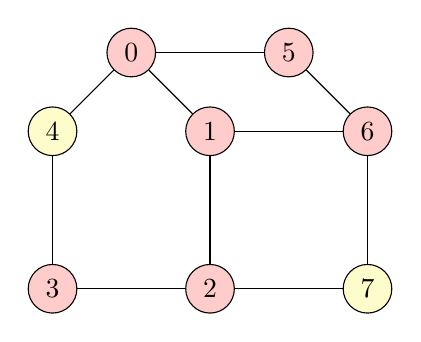
\begin{tikzpicture}[auto,node_style/.style={circle,draw=black,fill=green!20!},
           node_style_selected/.style={circle,draw=black,fill=red!20!},
           node_style_selected2/.style={circle,draw=black,fill=yellow!20!},
           edge_style/.style={draw=black}]
            \node[node_style_selected] (v0) at (1, 3)  {0};
            \node[node_style_selected] (v1) at (2, 2)  {1};
            \node[node_style_selected] (v2) at (2, 0)  {2};
            \node[node_style_selected] (v3) at (0, 0)  {3};
            \node[node_style_selected2] (v4) at (0, 2)  {4};
            \node[node_style_selected] (v5) at (3, 3)  {5};
            \node[node_style_selected] (v6) at (4, 2)  {6};
            \node[node_style_selected2] (v7) at (4, 0)  {7};
            \draw[edge_style]  (v0) edge node{} (v1);
            \draw[edge_style]  (v1) edge node{} (v2);
            \draw[edge_style]  (v2) edge node{} (v3);
            \draw[edge_style]  (v2) edge node{} (v7);
            \draw[edge_style]  (v3) edge node{} (v4);
            \draw[edge_style]  (v4) edge node{} (v0);
            \draw[edge_style]  (v0) edge node{} (v5);
            \draw[edge_style]  (v1) edge node{} (v6);
            \draw[edge_style]  (v5) edge node{} (v6);
            \draw[edge_style]  (v6) edge node{} (v7);
        \end{tikzpicture}
    }
    \end{column}
    \begin{column}{.5\textwidth}
     $S = \{1, 3, 5\}$ É Convexo?
    \begin{itemize}
        \item{$I^1{[}S{]}=\{1, 3, 5, 0, 2, 6 \}$}
        \item{$I^2{[}S{]}=I{[}I^1{[}S{]}{]}=\{1, 3, 5, 0, 2, 6, 4, 7\}$}
    \end{itemize}
    \end{column}
  \end{columns}
\end{frame}


\begin{frame}
\frametitle{Convexidade $P_3$}
\framesubtitle{Envoltória Convexa}
  \begin{columns}[T]
    \begin{column}{.5\textwidth}
    \centering
    \resizebox{\textwidth}{!}{%
        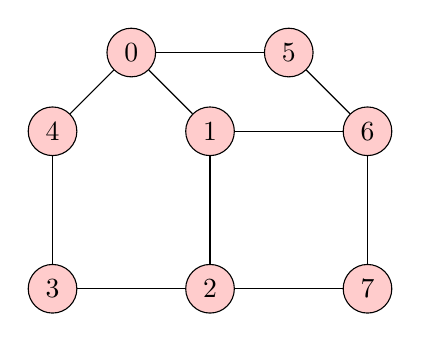
\begin{tikzpicture}[auto,node_style/.style={circle,draw=black,fill=green!20!},
           node_style_selected/.style={circle,draw=black,fill=red!20!},
           node_style_selected2/.style={circle,draw=black,fill=yellow!20!},
           edge_style/.style={draw=black}]
            \node[node_style_selected] (v0) at (1, 3)  {0};
            \node[node_style_selected] (v1) at (2, 2)  {1};
            \node[node_style_selected] (v2) at (2, 0)  {2};
            \node[node_style_selected] (v3) at (0, 0)  {3};
            \node[node_style_selected] (v4) at (0, 2)  {4};
            \node[node_style_selected] (v5) at (3, 3)  {5};
            \node[node_style_selected] (v6) at (4, 2)  {6};
            \node[node_style_selected] (v7) at (4, 0)  {7};
            \draw[edge_style]  (v0) edge node{} (v1);
            \draw[edge_style]  (v1) edge node{} (v2);
            \draw[edge_style]  (v2) edge node{} (v3);
            \draw[edge_style]  (v2) edge node{} (v7);
            \draw[edge_style]  (v3) edge node{} (v4);
            \draw[edge_style]  (v4) edge node{} (v0);
            \draw[edge_style]  (v0) edge node{} (v5);
            \draw[edge_style]  (v1) edge node{} (v6);
            \draw[edge_style]  (v5) edge node{} (v6);
            \draw[edge_style]  (v6) edge node{} (v7);
        \end{tikzpicture}
    }
    \end{column}
    \begin{column}{.5\textwidth}
     $S = \{1, 3, 5\}$ É Convexo?
    \begin{itemize}
        \item{$I^1{[}S{]}=\{1, 3, 5, 0, 2, 6 \}$}
        \item{$I^2{[}S{]}=I{[}I^1{[}S{]}{]}=\{1, 3, 5, 0, 2, 6, 4, 7\}$}
        \item{$I^3{[}S{]}=I{[}I^2{[}S{]}{]}=I^2{[}S{]}=\{0, 1, 2, 3, 4, 5, 6, 7\}$}
    \end{itemize}
    $H(S)=\{0, 1, 2, 3, 4, 5, 6, 7\}$
    \end{column}
  \end{columns}
\end{frame}


\begin{frame}
\frametitle{Convexidade $P_3$}
\framesubtitle{Envoltória Convexa}
\textit{Envoltória convexa:} $H(S)$ de um subconjunto $S$, é o menor conjunto convexo que contem S.
\end{frame}

\begin{frame}
\frametitle{Convexidade $P_3$}
\centering
\textbf{1º Parâmetro: Número Envoltório}
\end{frame}

\begin{frame}
\frametitle{Convexidade $P_3$}
\framesubtitle{Nº Envoltório}
 \begin{columns}[T]
    \begin{column}{.5\textwidth}
    \centering
    \resizebox{\textwidth}{!}{%
        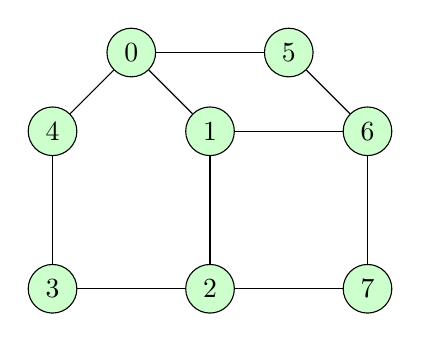
\begin{tikzpicture}[auto,
           node_style/.style={circle,draw=black,fill=green!20!},
           node_style_selected/.style={circle,draw=black,fill=red!20!},
           node_style_selected2/.style={circle,draw=black,fill=yellow!20!},
           edge_style/.style={draw=black}]
            \node[node_style] (v0) at (1, 3)  {0};
            \node[node_style] (v1) at (2, 2)  {1};
            \node[node_style] (v2) at (2, 0)  {2};
            \node[node_style] (v3) at (0, 0)  {3};
            \node[node_style] (v4) at (0, 2)  {4};
            \node[node_style] (v5) at (3, 3)  {5};
            \node[node_style] (v6) at (4, 2)  {6};
            \node[node_style] (v7) at (4, 0)  {7};
            \draw[edge_style]  (v0) edge node{} (v1);
            \draw[edge_style]  (v1) edge node{} (v2);
            \draw[edge_style]  (v2) edge node{} (v3);
            \draw[edge_style]  (v2) edge node{} (v7);
            \draw[edge_style]  (v3) edge node{} (v4);
            \draw[edge_style]  (v4) edge node{} (v0);
            \draw[edge_style]  (v0) edge node{} (v5);
            \draw[edge_style]  (v1) edge node{} (v6);
            \draw[edge_style]  (v5) edge node{} (v6);
            \draw[edge_style]  (v6) edge node{} (v7);
        \end{tikzpicture}
    }
    \end{column}
    \begin{column}{.5\textwidth}
        \begin{itemize}
            \item{$H(S)=V(G)$ $\Rightarrow$ $S$ é  um \textit{conjunto envoltório}}
            \item{$h(G)$ é a cardinalidade do menor conjunto envoltório}
        \end{itemize}
    \end{column}
  \end{columns}
\end{frame}

\begin{frame}
\frametitle{Convexidade $P_3$}
\framesubtitle{Nº Envoltório}
  \begin{columns}[T]
    \begin{column}{.5\textwidth}
    \centering
    \resizebox{\textwidth}{!}{%
        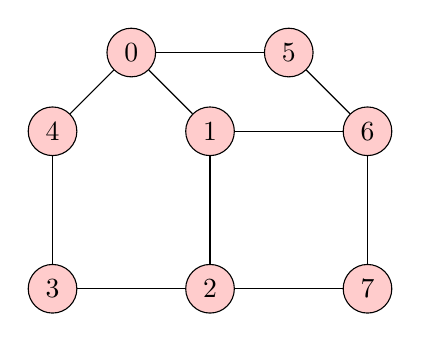
\begin{tikzpicture}[auto,node_style/.style={circle,draw=black,fill=green!20!},
           node_style_selected/.style={circle,draw=black,fill=red!20!},
           node_style_selected2/.style={circle,draw=black,fill=yellow!20!},
           edge_style/.style={draw=black}]
            \node[node_style_selected] (v0) at (1, 3)  {0};
            \node[node_style_selected] (v1) at (2, 2)  {1};
            \node[node_style_selected] (v2) at (2, 0)  {2};
            \node[node_style_selected] (v3) at (0, 0)  {3};
            \node[node_style_selected] (v4) at (0, 2)  {4};
            \node[node_style_selected] (v5) at (3, 3)  {5};
            \node[node_style_selected] (v6) at (4, 2)  {6};
            \node[node_style_selected] (v7) at (4, 0)  {7};
            \draw[edge_style]  (v0) edge node{} (v1);
            \draw[edge_style]  (v1) edge node{} (v2);
            \draw[edge_style]  (v2) edge node{} (v3);
            \draw[edge_style]  (v2) edge node{} (v7);
            \draw[edge_style]  (v3) edge node{} (v4);
            \draw[edge_style]  (v4) edge node{} (v0);
            \draw[edge_style]  (v0) edge node{} (v5);
            \draw[edge_style]  (v1) edge node{} (v6);
            \draw[edge_style]  (v5) edge node{} (v6);
            \draw[edge_style]  (v6) edge node{} (v7);
        \end{tikzpicture}
    }
    \end{column}
    \begin{column}{.5\textwidth}
    \begin{itemize}
        \item{$S = \{1, 3, 5\}$}
        \item{$H(S)=\{0, 1, 2, 3, 4, 5, 6, 7\}=V(G)$}
        \item{Não existe conjunto envoltório de cardinalidade 1 ou 2 para o grafo}
        \item{h(G)=3}
    \end{itemize}
    \end{column}
  \end{columns}
\end{frame}

\begin{frame}
\frametitle{Convexidade $P_3$}
\centering
\textbf{2º Parâmetro: Número de Carathéodory}
\end{frame}

\begin{frame}
\frametitle{Convexidade $P_3$}
\framesubtitle{Nº de Caratheodory}
 \begin{columns}[T]
    \begin{column}{.5\textwidth}
    \centering
    \resizebox{\textwidth}{!}{%
        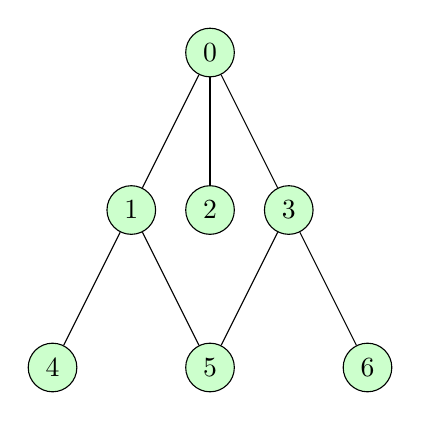
\begin{tikzpicture}
        [auto,
         node_style/.style={circle,draw=black,fill=green!20!},
         node_style_selected/.style={circle,draw=black,fill=red!20!},
         node_style_selected2/.style={circle,draw=black,fill=yellow!20!},
         edge_style/.style={draw=black}]
            \node[node_style] (v0) at (2, 4)  {0};
            \node[node_style] (v1) at (1, 2)  {1};
            \node[node_style] (v2) at (2, 2)  {2};
            \node[node_style] (v3) at (3, 2)  {3};
            \node[node_style] (v4) at (0, 0)  {4};
            \node[node_style] (v5) at (2, 0)  {5};
            \node[node_style] (v6) at (4, 0)  {6};
            \draw[edge_style]  (v0) edge node{} (v1);
            \draw[edge_style]  (v0) edge node{} (v2);
            \draw[edge_style]  (v0) edge node{} (v3);
            \draw[edge_style]  (v1) edge node{} (v4);
            \draw[edge_style]  (v1) edge node{} (v5);
            \draw[edge_style]  (v3) edge node{} (v5);
            \draw[edge_style]  (v3) edge node{} (v6);
        \end{tikzpicture}%
    }
    \end{column}
    \begin{column}{.5\textwidth}
        $S=\{4, 5, 6\}$
    \end{column}
  \end{columns}
\end{frame}

\begin{frame}
\frametitle{Convexidade $P_3$}
\framesubtitle{Nº de Caratheodory}
 \begin{columns}[T]
    \begin{column}{.5\textwidth}
    \centering
    \resizebox{\textwidth}{!}{%
        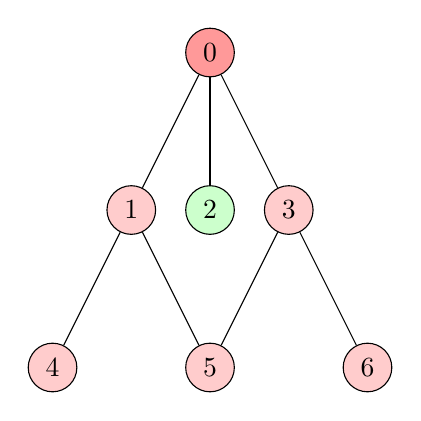
\begin{tikzpicture}
        [auto,
         node_style/.style={circle,draw=black,fill=green!20!},
         node_style_selected/.style={circle,draw=black,fill=red!20!},
         node_style_selected2/.style={circle,draw=black,fill=red!40!},
         edge_style/.style={draw=black}]
            \node[node_style_selected2] (v0) at (2, 4)  {0};
            \node[node_style_selected] (v1) at (1, 2)  {1};
            \node[node_style] (v2) at (2, 2)  {2};
            \node[node_style_selected] (v3) at (3, 2)  {3};
            \node[node_style_selected] (v4) at (0, 0)  {4};
            \node[node_style_selected] (v5) at (2, 0)  {5};
            \node[node_style_selected] (v6) at (4, 0)  {6};
            \draw[edge_style]  (v0) edge node{} (v1);
            \draw[edge_style]  (v0) edge node{} (v2);
            \draw[edge_style]  (v0) edge node{} (v3);
            \draw[edge_style]  (v1) edge node{} (v4);
            \draw[edge_style]  (v1) edge node{} (v5);
            \draw[edge_style]  (v3) edge node{} (v5);
            \draw[edge_style]  (v3) edge node{} (v6);
        \end{tikzpicture}%
    }
    \end{column}
    \begin{column}{.5\textwidth}
        $S=\{4, 5, 6\}$
        \begin{itemize}
            \item{$H(S)=\{0,1, 3, 4, 5, 6\}$}
            \item{$\partial H(S)=\{0\}$}
        \end{itemize}
    \end{column}
  \end{columns}
\end{frame}

\begin{frame}
\frametitle{Convexidade $P_3$}
\framesubtitle{Nº de Caratheodory}
\begin{columns}[T]
\begin{column}{.5\textwidth}
\centering
\resizebox{\textwidth}{!}{%
    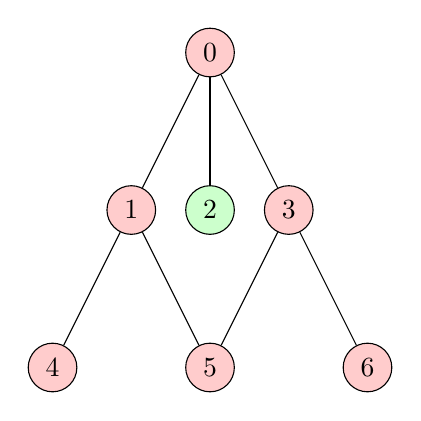
\begin{tikzpicture}
    [auto,
     node_style/.style={circle,draw=black,fill=green!20!},
     node_style_selected/.style={circle,draw=black,fill=red!20!},
     node_style_selected2/.style={circle,draw=black,fill=yellow!20!},
     edge_style/.style={draw=black}]
        \node[node_style_selected] (v0) at (2, 4)  {0};
        \node[node_style_selected] (v1) at (1, 2)  {1};
        \node[node_style] (v2) at (2, 2)  {2};
        \node[node_style_selected] (v3) at (3, 2)  {3};
        \node[node_style_selected] (v4) at (0, 0)  {4};
        \node[node_style_selected] (v5) at (2, 0)  {5};
        \node[node_style_selected] (v6) at (4, 0)  {6};
        \draw[edge_style]  (v0) edge node{} (v1);
        \draw[edge_style]  (v0) edge node{} (v2);
        \draw[edge_style]  (v0) edge node{} (v3);
        \draw[edge_style]  (v1) edge node{} (v4);
        \draw[edge_style]  (v1) edge node{} (v5);
        \draw[edge_style]  (v3) edge node{} (v5);
        \draw[edge_style]  (v3) edge node{} (v6);
    \end{tikzpicture}%
}
\end{column}
\begin{column}{.5\textwidth}
$S=\{4, 5, 6\}$
\begin{itemize}
\item{$H(S)=\{0,1, 3, 4, 5, 6\}$}
\item{$H(S \setminus \{4\})=\{5, 6, 3\}$}
\item{$H(S \setminus \{5\})=\{4, 6\}$}
\item{$H(S \setminus \{6\})=\{4, 5, 1\}$}
\item{$\partial H(S)=H(S) \setminus $(H(S \setminus \{4\}) \cup H(S \setminus \{5\}) \cup H(S\setminus \{6\}))$}
\item{$\partial H(S)=\{0\}$}
\end{itemize}
\end{column}
\end{columns}
\end{frame}

\begin{frame}
\frametitle{Convexidade $P_3$}
\framesubtitle{Nº de Caratheodory}
 \begin{columns}[T]
    \begin{column}{.5\textwidth}
    \centering
    \resizebox{\textwidth}{!}{%
        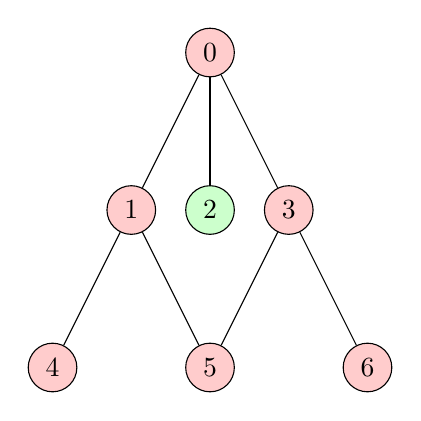
\begin{tikzpicture}
        [auto,
         node_style/.style={circle,draw=black,fill=green!20!},
         node_style_selected/.style={circle,draw=black,fill=red!20!},
         node_style_selected2/.style={circle,draw=black,fill=yellow!20!},
         edge_style/.style={draw=black}]
            \node[node_style_selected] (v0) at (2, 4)  {0};
            \node[node_style_selected] (v1) at (1, 2)  {1};
            \node[node_style] (v2) at (2, 2)  {2};
            \node[node_style_selected] (v3) at (3, 2)  {3};
            \node[node_style_selected] (v4) at (0, 0)  {4};
            \node[node_style_selected] (v5) at (2, 0)  {5};
            \node[node_style_selected] (v6) at (4, 0)  {6};
            \draw[edge_style]  (v0) edge node{} (v1);
            \draw[edge_style]  (v0) edge node{} (v2);
            \draw[edge_style]  (v0) edge node{} (v3);
            \draw[edge_style]  (v1) edge node{} (v4);
            \draw[edge_style]  (v1) edge node{} (v5);
            \draw[edge_style]  (v3) edge node{} (v5);
            \draw[edge_style]  (v3) edge node{} (v6);
        \end{tikzpicture}%
    }
    \end{column}
    \begin{column}{.5\textwidth}
        $S=\{4, 5, 6\}$
        \begin{itemize}
            \item{$H(S)=\{0,1, 3, 4, 5, 6\}$}
            \item{$\partial H(S)=\{0\}$}
            \item{$\partial H(S)$ não é vazio}
            \item{S é um conjunto de Carathéodory}
        \end{itemize}
    \end{column}
  \end{columns}
\end{frame}

\begin{frame}
\frametitle{Convexidade $P_3$}
\framesubtitle{Nº de Caratheodory}
 \begin{columns}[T]
    \begin{column}{.5\textwidth}
    \centering
    \resizebox{\textwidth}{!}{%
        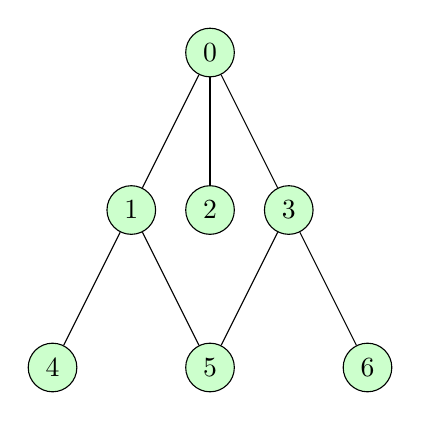
\begin{tikzpicture}
        [auto,
         node_style/.style={circle,draw=black,fill=green!20!},
         node_style_selected/.style={circle,draw=black,fill=red!20!},
         node_style_selected2/.style={circle,draw=black,fill=yellow!20!},
         edge_style/.style={draw=black}]
            \node[node_style] (v0) at (2, 4)  {0};
            \node[node_style] (v1) at (1, 2)  {1};
            \node[node_style] (v2) at (2, 2)  {2};
            \node[node_style] (v3) at (3, 2)  {3};
            \node[node_style] (v4) at (0, 0)  {4};
            \node[node_style] (v5) at (2, 0)  {5};
            \node[node_style] (v6) at (4, 0)  {6};
            \draw[edge_style]  (v0) edge node{} (v1);
            \draw[edge_style]  (v0) edge node{} (v2);
            \draw[edge_style]  (v0) edge node{} (v3);
            \draw[edge_style]  (v1) edge node{} (v4);
            \draw[edge_style]  (v1) edge node{} (v5);
            \draw[edge_style]  (v3) edge node{} (v5);
            \draw[edge_style]  (v3) edge node{} (v6);
        \end{tikzpicture}%
    }
    \end{column}
    \begin{column}{.5\textwidth}
        $S=\{4, 5, 6\}$
        \begin{itemize}
            \item{$\partial H(S)=H(S) \setminus \bigcup _{u \in S} H(S \setminus \{u\})$}
            \item{$\partial H(S) \ne \emptyset$ $\Rightarrow$ $S$ é  um \textit{conjunto de Carathéodory}}
            \item{$c(G)$ é equivalente a cardinalidade do maior conjunto de Carathéodory}
            \item{Não existe conjunto de Carathéodory maior que 3 para o grafo}
            \item{$c(G)$=3}
            %\item{$c(G)$ é a cardinalidade do maior conjunto de Carathéodory}
        \end{itemize}
    \end{column}
  \end{columns}
\end{frame}

\begin{frame}
\frametitle{Convexidade $P_3$}
\framesubtitle{Nº de Caratheodory}
Número de Carathéodory:
\begin{itemize}
\item{Se $\partial H(S)=H(S) \setminus \bigcup _{u \in S} H(S \setminus \{u\})$,
é não vazio, então $S$ é um \textit{conjunto de Carathéodory}}
\item{O \textit{número de Carathéodory} $c(G)$ é o menor inteiro $c$,
para o qual todo $u \in H(S)$, existe um conjunto $F \subseteq  S$,
com $|F| \le c$ e $u \in H(F)$}
\item{Esta definição permite uma  forma alternativa,
o número de Carathéodory é a maior cardinalidade de um conjunto de Carathéodory}
\end{itemize}
\end{frame}
